\documentclass{standalone}

\usepackage{blox}
\usepackage{tikz}
\usetikzlibrary{positioning}

\begin{document}
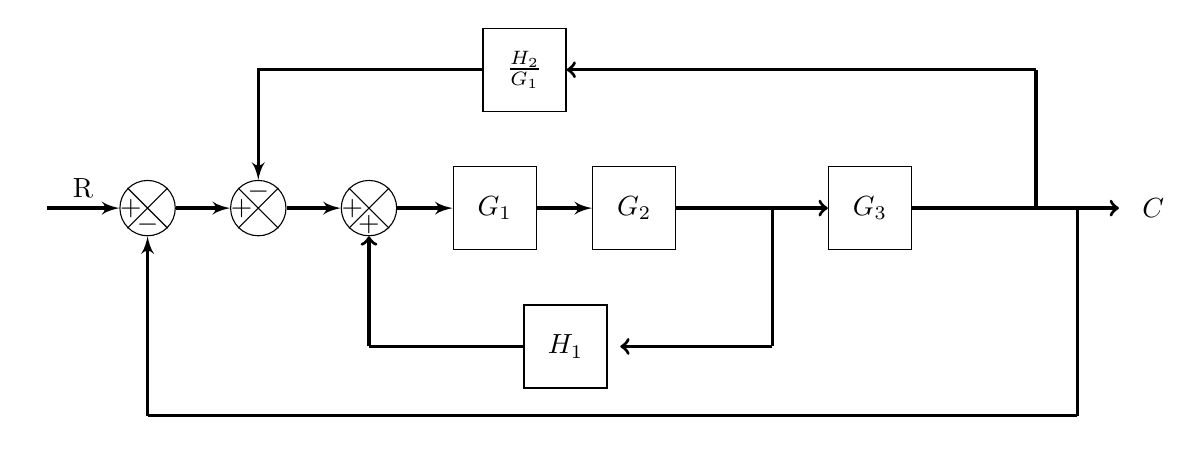
\begin{tikzpicture}
%\bXLineStyle{red, dotted}
\bXLineStyle{very thick}
\bXInput{A}
\bXComp{B}{A}
\bXLink[R]{A}{B}
\bXCompa{C}{B}
\bXLink{B}{C}
\bXSumb{D}{C}
\bXLink{C}{D}
\bXBloc[2]{E}{$G_1$}{D}
\bXLink{D}{E}
\bXBloc[2]{F}{$G_2$}{E}
\bXLink{E}{F}

\bXBranchx[5]{F}{FX1}

\bXBranchy[5]{FX1}{FDown1}
\draw[-,very thick] (F) -- (FX1.center);
\draw[-,very thick] (FX1.center) -- (FDown1.center);
\bXBranchx[-5.5]{FDown1}{FRight1}
\draw[->,very thick] (FDown1.center) -- (FRight1.center);
\bXBloc[-3.5]{H1}{$H_1$}{FRight1}
\bXBranchy[5]{D}{DDown1}
\draw[->,very thick] (DDown1.center) -- (D);
\draw[-,very thick] (H1) -- (DDown1.center);

\bXBloc[2]{G}{$G_3$}{FX1}
%\draw[-,very thick]  (F)  -- (FX1);
\draw[->,very thick] (F) -- (G);

\bXBranchx[3]{G}{GX1}
\bXBranchx[3]{GX1}{GX2}
\draw[-,very thick] (G) -- (GX2);
\bXBranchx[3]{GX2}{GX3}
\bXBranchy[-5]{GX2}{GUp1}

\bXBranchx[1.5]{GX2}{GX4}
\bXBranchy[7.5]{GX4}{GDown1}
%\draw[-,very thick] (G) -- (GX1.center);
%\draw[-,very thick] (G) -- (GX1.center);
%\draw[-,very thick] (GX1.center) -- (GUp1.center);
%\bXLinkxy{GX1}{GUp1}
\draw[-,very thick] (GX1.center) -- (GX2.center);
\draw[-,very thick] (GX2.center) -- (GUp1.center);
\draw[->,very thick] (GX2.center) -- (GX3.center);
\node[right = 0.05cm of GX3] (end) {$C$};

\draw[-,very thick] (GX4.center) -- (GDown1.center);

\bXBranchy[7.5]{B}{BDown1}
\bXLink{BDown1.center}{B}
\draw[-,very thick] (GDown1.center) -- (BDown1.center);


%% Top Part

\bXBranchx[-20]{GUp1}{GLUp1}
\bXBloc[-0]{BlockHG}{$\frac{H_2}{G_1}$}{GLUp1}
\draw[->,very thick] (GUp1.center) -- (BlockHG);
\bXLinkxy{BlockHG}{C}
\end{tikzpicture}
\end{document}